\documentclass{minimal}

\usepackage{bm}
\usepackage{tikz}
\usetikzlibrary{
	arrows.meta,
	decorations.pathmorphing,
	backgrounds,
	positioning,
	fit,
	petri,
	shapes.misc,
	graphs,
	quotes,
	decorations.pathreplacing,
	calc,
}

\tikzset{unobserved/.style={
		% The shape:
		circle,
		% The size:
		minimum size=12mm,
		% The border:
		semithick,
		draw=black,
}}

\begin{document}
	
\pagestyle{empty}

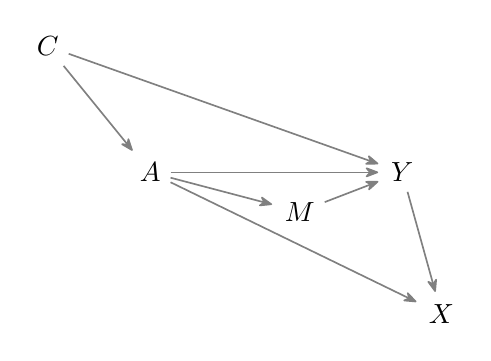
\begin{tikzpicture}[
	>= {Stealth[round]},semithick,black!50,
	text=black, 
	node distance = 1.6cm, 
	every new ->/.style={shorten >=1pt},
	graphs/every graph/.style={edges=rounded corners}
	]
	
	%% line 1
	\node (C)  {$C$};		
	
	%% line 2
	\node (empty11) [below of=C] { };
	\node (A) [right of=empty11,xshift=-3mm]  {$A$};		
	\node (M) [right of=A,xshift=3mm,yshift=-5mm] {$M$};
	\node (Y) [right of=M,xshift=-3mm,yshift=5mm] {$Y$};

	%% line 3
	\node (X) [below of=Y,xshift=5mm,yshift=-2mm]  {$X$};		
	
	%% from time=0 nodes
	\draw[->,shorten >=1pt] (C) to (A);
	\draw[->,shorten >=1pt] (C) to (Y);
	\draw[->,shorten >=1pt] (A) to (M);
	\draw[->,shorten >=1pt] (A) to (Y);	
	\draw[->,shorten >=1pt] (A) to (X);	
	\draw[->,shorten >=1pt] (M) to (Y);
	\draw[->,shorten >=1pt] (Y) to (X);
	
\end{tikzpicture}

\end{document}
